\chapter{Analýza}
%% TODO: zde napsat prehledovy text o tom, co vsechno tato kapitola obsahuje

%% Analýza a návrh implementace (včetně diskuse různých alternativ a volby implementačního prostředí).

%% V části analýzy provést rozbor jednotlivých principů + výsledky rešerší - využívat hojně informace z článků a důsledně citovat zdroje

\section{Analýza principů objektového návrhu}

%% PRINCIPY versus PATTERNY -> citovat clanek

\subsection{Analyzované principy}
Ukázkové návrhové principy analyzované v rámci této práce jsou znázorněny na obrázku \ref{analyzed_principles}. Poznamenejme, že tzv. Demeterův zákon je speciálním případem pravidla pro \uv{low coupling}.

\begin{figure}[h!]
  \centering
  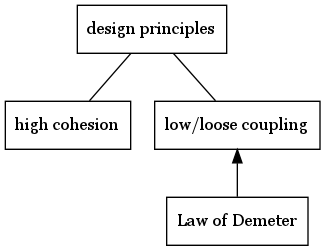
\includegraphics[width=0.5\textwidth]{./graphs/oop_design_principles.png}
  \caption{Znázornění analyzovaných návrhových principů.\label{analyzed_principles}}
\end{figure}

% TODO: v rámci každého návrhového principu uvést příklad porušení
% tohoto principu (případně i příklad, který tento princip dodržuje)

% Příklad pravidla:
% ``Třídy z balíčku A nesmí záviset na jiných konkrétních třídách, ale nejvýše na rozhraních balícků B.''
%  (programování proti rozhraní namísto proti kokrétní implementaci)"

\subsubsection{Low coupling/dependency (nízká závislost/vazba)}
Důležitou návrhovou zásadou je snaha snížit provázanost modulů na minimum. Je možné kategorizovat způsob provázanosti modulů do různých skupin. Následující přehled je převzat z \cite{wiki:coupling} (ještě jemnější dělení je uváděno v \cite{STVR:STVR162}).

\begin{itemize}
\item\emph{Content coupling (nejvyšší forma závislosti)} -- závislost na obsahu modulu -- jeden modul modifikuje nebo se spoléhá na vnitřní fungování jiného modulu (např. přístup k lokálním datům jiného modulu). V důsledku platí, že změní-li se způsob, kterým tento druhý modul produkuje data (umístění, typ, časování), povede to zcela jiste ke změnám v závislém modulu.
\item\emph{Common coupling} -- dva moduly sdílí stejná globální data (např. globální proměnnou), změna sdíleného globálního zdroje implikuje změny všech modulů, které je používají.
\item\emph{External coupling} -- dva moduly sdílí externě definovaný (standardizovaný) datový formát, komunikační protokol nebo rozraní zařízení.
\item\emph{Control coupling} -- jeden modul kontroluje tok druhého tím, že mu posílá informaci o tom, co má konat (např. předání \uv{to-do} příznaku).
  % TODO: CLARIFY
\item\emph{Stamp coupling (Data-structured coupling)} -- mdouly sdílí složenou datovou strukturu a používají pouze její (často odlišnou) část (např. předávání kompletního záznamu funkci, která z něj potřebuje pouze jedno pole). Tato vazba může vést ke změně způsobu, kterým modul čte záznam, protože pole, které tento modul nepotřebuje bylo modifikováno.
  % Stamp coupling is when modules share a composite data structure and use only a part of it, possibly a different part (e.g., passing a whole record to a function that only needs one field of it). This may lead to changing the way a module reads a record because a field that the module doesn't need has been modified.
\item\emph{Data coupling} -- moduly sdílí data pomocí parametrů. Každý parametr je elementární datový typ a jedná se o jediná data, která jsou sdílená (např. předávání celočíselné hodnoty funkci, která spočítá jeho druhou mocninu).
\item\emph{Message coupling (nejnižší forma závislosti)} -- provázanost modulů pouze pomocí zpráv, jedná se o nejnižší úroveň závislosti. Lze jí dosáhnout pomocí decentralizace stavu (u objektů), kde je komunikace dosahováno pomocí parametrů nebo předávání zpráv (\uv{message passing}).
\item\emph{No coupling} -- žádná závislost -- moduly spolu vůbec nekomunikují.
\end{itemize}

%% TODO: sort
%% ## Typy závislostí mezi třídami

%% * třída A dědí ze třídy B
%% * třída A provádí instanciaci třídy B
%% * třída A používá existující intanci třídy B (pracuje s referencí na tuto třídu)

%% Na základě těchto závislostí lze sestavit orientovaný graf. Hrany budeme dále klasifikovat podle toho, o jakou závislost se jedná (dědičnost vs. vyvolání metody).

\subsubsection{High cohesion}

\subsubsection{Law of Demeter}

Existuje několik forem Demeterova zákona \cite{35588}, které jsou vhodné pro různé oblasti aplikace. Tyto typy jsou znázorněny na obrázku \ref{demeter_law_types}.

\begin{figure}[h!]
  \centering
  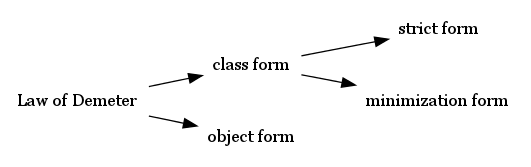
\includegraphics[width=0.7\textwidth]{./graphs/demeter_law_types.png}
  \caption{Formy Demeterova zákona.\label{demeter_law_types}}
\end{figure}

Pro statickou analýzu lze použít \uv{class} formu Demeterova zákona.

\subsection{Ukázky kódu porušujících některá z pravidel}

\subsubsection{Porušení principu law of Demeter}

%% TODO: use some highlighter
%% TODO: add example of demeter law violation from paper notes
\begin{verbatim}
package handlers;

public class ...

\end{verbatim}

\section{Analýza problematiky v jazyce Java}

\subsection{Statický model programu v Javě}
TODO: pojednání o tom, co všechno může být modelem programu (ast, graf, FSM, programovací jazyky, atd)

\subsubsection{Struktura softwarového projektu v Javě}

% TODO: sort and rephrase
\begin{itemize}
\item\verb+*.java+ soubory - v gramatice programovacího jazyka Java 1.5 představují top-level element CompilationUnit \emph{\{(TODO: binární součásti projektu? class files?)\}}
\item další soubory - resources, documentation, \ldots
\end{itemize}

Pro naše potřeby jsou důležité v podstatě pouze kompilační jednotky (java soubory) projektu.

Statický pohled na program - neuvažujeme běh programu. Pracujeme nad definicemi tříd, nikoliv nad jejich instancemi v paměti JVM.

% TODO: aktualizovat -> v konecnem dusledku budeme pracovat i nad projekty v jazyku 1.6 (protoze nam to rozhrani umoznuje)
Budeme pracovat nad gramatikou jazyka Java 1.5. Java verze 6 se liší pouze úpravou standardních API poskytovaných platformou Java. Jazyk jako takový zůstává stejný.

\subsubsection{Syntaktické elementy programovacího jazyka Java}
Grafické znázornění základních syntaktických elementů, jejichž struktura a názvy jsou převzaty z \cite{Gosling:2005:JLS:1036643}, je na obrázku \ref{toplevel_elements}.
% TODO: write some better accompanying text
\begin{figure}[h!]
  \centering
  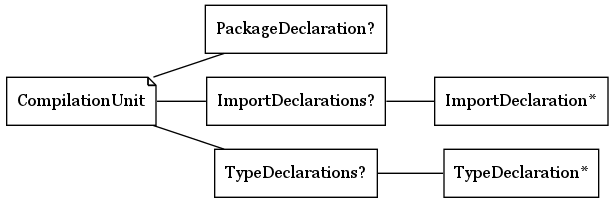
\includegraphics[width=\textwidth]{./graphs/java_top_elements.png}
  \caption{Struktura základních syntaktických elementů programovacího jazyka Java.\label{toplevel_elements}}
\end{figure}

Pro analýzu založenou na vyhledávání závislostí mezi třídami pro nás bude nejdůležitější syntaktický element \emph{TypeDeclaration}. Tento neterminální symbol se dále přepisuje na symboly uvedené na obrázku \ref{type_declaration_options}.

\begin{figure}[h!]
  \centering
  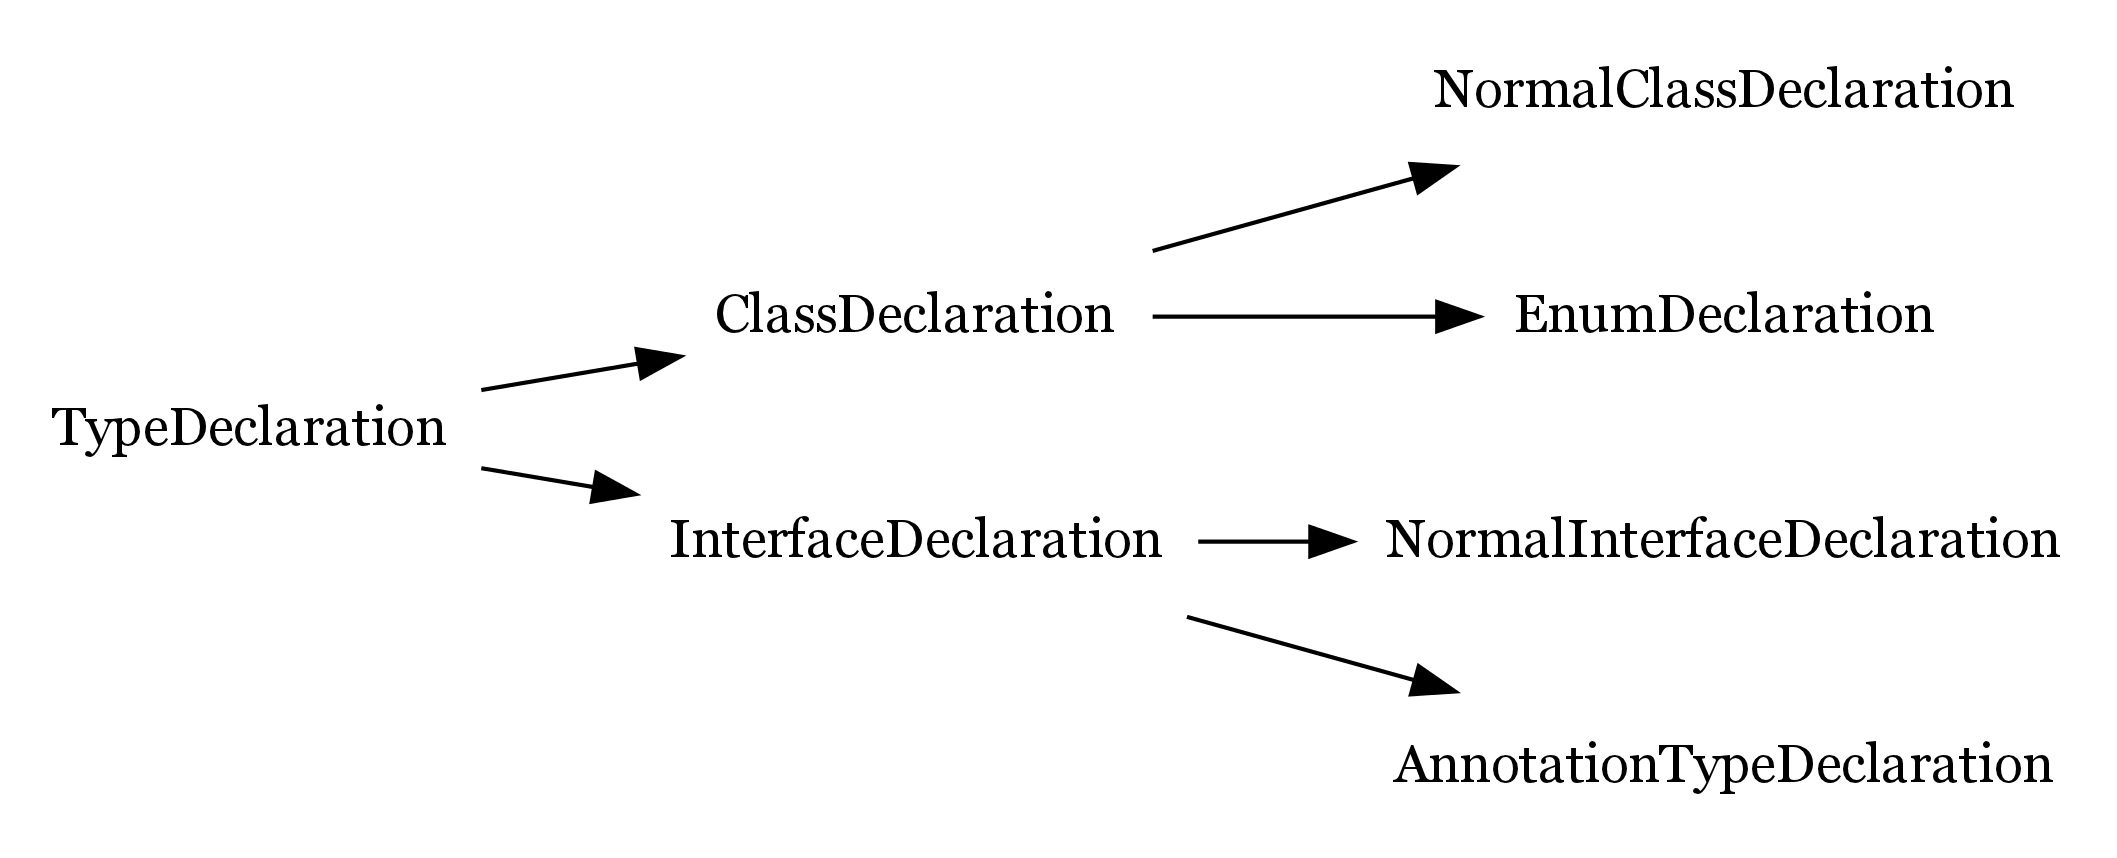
\includegraphics[width=\textwidth]{./graphs/toplevel_types.png}
  \caption{Rozklad elementu TypeDeclaration.\label{type_declaration_options}}
\end{figure}

%% TODO: zatridit tyto syntakticke elementy, ke kazdemu napsat, jak se bude zpracovavat
%% interfaces
%% enums
%% annotations

%% Modifikátory přístupu (private, public, protected, package private) nám umožní "ořezat" graf závislosti tříd. Je ale možné, že pro některé druhy analýzy bude toto nežádoucí.

%% ## Speciální případy:

%% * statické třídy
%% * statické metody
%% * vnitřní třídy

\subsection{Existující nástroje pro zpracování zdrojových kódů v jazyku Java}

TODO: write some leading text 

Možnosti zpracovávání kódu:

TODO: roztřídit a vyházet nesmysly (e.g. JABA, apod.)

TODO: použít jinou vhodnější strukturu místo itemize

\begin{itemize}
\item vlastní hand-written lexikální a syntaktický analyzátor (zbytečně náročné)
\item parser vygenerovaný pomocí některého z dostupných compiler-compiler systémů
  \begin{itemize}
  \item tyto systémy na základě vstupní gramatiky vygenerují frontend pro překladač
  \item lze specifikovat různé akce, které jsou navázány na události vyvolané v průběhu syntaktické analýzy
  \item \emph{JavaCC}
    \begin{itemize}
    \item \href{http://www.cs.purdue.edu/homes/hosking/352/javaccdocs/docindex.html}{http://www.cs.purdue.edu/homes/hosking/352/javaccdocs/docindex.html}
    \end{itemize}
  \item \emph{JastAdd}
    \begin{itemize}
    \item \href{http://jastadd.org/}{http://jastadd.org/}
    \end{itemize}
  \item \emph{JLex}
    \begin{itemize}
    \item A Lexical Analyzer Generator for Java(TM)
    \item \href{http://www.cs.princeton.edu/~appel/modern/java/JLex/}{http://www.cs.princeton.edu/~appel/modern/java/JLex/}
    \end{itemize}
  \item JFlex
    \begin{itemize}
    \item The Fast Scanner Generator for Java
    \item \href{http://jflex.de/}{http://jflex.de/}
    \end{itemize}
  \item JABA
    \begin{itemize}
    \item \href{http://pleuma.cc.gatech.edu/aristotle/Tools/jaba.html}{http://pleuma.cc.gatech.edu/aristotle/Tools/jaba.html}
    \item Java Architecture for Bytecode Analysis
    \item nepoužitelné - dostupná pouze binární verze pro Solaris
    \item pravděpodobně se dále nevyvíjí
    \end{itemize}
  \end{itemize}
\item použití vhodné knihovny
  \begin{itemize}
  \item JavaParser
    \begin{itemize}
    \item \href{http://code.google.com/p/javaparser/}{http://code.google.com/p/javaparser/}
    \item projekt na GoogleHosting 
    \item v podstatě gramatika pro JJTree vytvářející strom tříd a objektů, který je možné procházet pomocí visitor patternu
    \end{itemize}
  \end{itemize}
\item použití prostředků platformy NetBeans 
  \begin{itemize}
  \item Retouche API
  \item \href{http://bits.netbeans.org/6.9.1/javadoc/}{http://bits.netbeans.org/6.9.1/javadoc/}
  \end{itemize}
\item použití prostředků poskytovaných platformou Java 6 (Sun verze) \cite{source_code_analysis_corejavatechtips}
  \begin{itemize}
  \item \emph{JSR 199 -- Java Compiler API}
    \begin{itemize}
    \item volání překladače jazyka Java pomocí API ze zdrojového kódu programu
    \item balíček \verb+javax.tools+
    \end{itemize}
  \item \emph{JSR 269 -- Pluggable Annotation Processing API}
    \begin{itemize}
    \item přidání vlastního kódu pro zpracovávání anotací (resp. celého zdrojového kódu) do instance překladače
    \item balíček \verb+javax.annotation.processing+ -- zpracovávání anotací
    \item balíček \verb+javax.lang.model+ -- třídy poskytující model pro syntaktické elementy jazyka Java
    \end{itemize}
  \item \emph{Compiler Tree API}
    \begin{itemize}
    \item nestandardní rozšíření Java JDK
    \item \href{http://download.oracle.com/javase/6/docs/jdk/api/javac/tree/index.html}{http://download.oracle.com/javase/6/docs/jdk/api/javac/tree/index.html}
    \item balíček \verb+com.sun.source.tree+ -- poskytuje rozhraní pro reprezentaci zdrojového kódu jako AST
    \item balíček \verb+com.sun.source.util+ -- poskytuje rozhraní pro operace nad AST
    \end{itemize}
  \end{itemize}
\end{itemize}

\section{Existující nástroje pro statickou analýzu kódu v Javě}
\label{analysis-existing_tools}
% TODO: do background research on positives and negatives of these tools
% TODO: v rychlosti zopakovat rešerši na nové nástroje a konkrétní vlastnosti, které jsou důležité pro tuto práci

\subsection{JDepend}

\begin{itemize}
\item \href{http://www.clarkware.com/software/JDepend.html}{http://www.clarkware.com/software/JDepend.html}
\item nástroj pro testování kvality návrhu
\item pracuje nad \verb+*.class+ soubory (získává data z bytekódu)
\end{itemize}

\subsection{QJ-Pro}
\begin{itemize}
\item \href{http://qjpro.sourceforge.net}{http://qjpro.sourceforge.net}
\end{itemize}

\subsection{DP-Miner}
\begin{itemize}
\item \href{http://www.utdallas.edu/~yxz045100/DesignPattern/DP\_Miner/}{http://www.utdallas.edu/~yxz045100/DesignPattern/DP\_Miner/}
\item hledání návrhových vzorů v existujících projektech
\item článek: Jing Dong and Yajing Zhao, Experiments on Design Pattern Discovery \\ (\href{http://www.utdallas.edu/~jdong/papers/PROMISE07.pdf}{http://www.utdallas.edu/~jdong/papers/PROMISE07.pdf})
\end{itemize}

\subsection{Macker}
\begin{itemize}
\item \href{http://innig.net/macker/}{http://innig.net/macker/}
\item build-time architectural rule checking utility for Java developers
\item zpracovává \verb+*.class+ soubory (bytekód)
\end{itemize}

TODO: přidat

\begin{itemize}
\item CheckStyle -- \href{http://checkstyle.sourceforge.net/}{http://checkstyle.sourceforge.net/}
\item PMD -- \href{http://pmd.sourceforge.net/}{http://pmd.sourceforge.net/}
\end{itemize}
